\documentclass[10pt]{article}
%%%%%%%%%%%%%%%%%%%%%%%%%%%%%%%%%%%%%%%%
\usepackage{amsmath}
\usepackage{verbatim}
\usepackage[usenames,dvipsnames]{color}
\usepackage{ulem}
\usepackage{setspace}
\usepackage{lscape}
\usepackage{longtable}
\usepackage[top=1.25in,bottom=1.5in,left=1in,right=1.5in,landscape]{geometry}
\usepackage{graphicx}
\usepackage{epstopdf}
\usepackage[usenames,dvipsnames]{pstricks}
\usepackage{epsfig}
\usepackage{pstricks-add}
\usepackage{pst-node}
\usepackage{fancyhdr}
\usepackage[absolute,showboxes]{textpos}

%TCIDATA{OutputFilter=LATEX.DLL}
%TCIDATA{Version=5.00.0.2552}
%TCIDATA{<META NAME="SaveForMode" CONTENT="1">}
%TCIDATA{Created=Thursday, August 28, 2003 13:38:44}
%TCIDATA{LastRevised=Thursday, August 14, 2008 15:20:27}
%TCIDATA{<META NAME="GraphicsSave" CONTENT="32">}
%TCIDATA{<META NAME="DocumentShell" CONTENT="Standard LaTeX\Blank - Standard LaTeX Article">}
%TCIDATA{Language=American English}
%TCIDATA{CSTFile=LaTeX article (bright).cst}

\setcounter{MaxMatrixCols}{10}

\newenvironment{proof}[1][Proof]{\noindent\textbf{#1.} }{\ \rule{0.5em}{0.5em}}
\setlength{\columnsep}{.2in}

\renewcommand{\labelitemii}{$\cdot$}

\pagestyle{fancy} \fancyhead{} \fancyfoot{} \rfoot{} \lfoot{}

\newcommand{\slide}[2]{
\begin{textblock}{11}(0,0)
\textcolor{Black}{\textbf{\huge \rule{0pt}{1in} \raisebox{.2in}{#1}}}
\end{textblock}
\begin{Large} \noindent
#2
\end{Large}
\vfill \pagebreak}

\setlength{\TPHorizModule}{1in}
\setlength{\TPVertModule}{1in}
\textblockcolour{Yellow}
\renewcommand{\headrulewidth}{0pt}



\begin{document}
\onehalfspacing 

\lfoot{Growth and Development} \rfoot{Economic Growth}

\slide{Growth versus Development}{The Romer and Schumpeterian models define the long-run trend growth rate. But they do not necessarily tell us whether a country is rich or poor. Why do some countries not use the same level of technology as others?

\vspace{.25in}\noindent Adapt the Romer model to allow for differences in development. Let
\begin{equation}
Y = L^{1-\alpha}\int_0^{h} x_j^{\alpha} dj
\end{equation}
be final goods production. Now the country uses $h$ varieties of intermediate good, rather than $A$. $h$ indexes how much technology a country can adopt at one time. Higher $h$, more technology.

\vspace{.25in}\noindent As before, intermediate goods are produced by monopolists who use capital to produce them. We presume then that
\begin{equation}
K = \int_0^{h} x_j dj 
\end{equation}
and that all $x_j = x$ so
\begin{equation}
K = h x
\end{equation}

}

\slide{Aggregate production and Capital}{Knowing $K = hx$, and the final goods production function, we have
\begin{equation}
Y = L^{1-\alpha}\int_0^{h} \left(\frac{K}{h}\right)^{\alpha} dj = L^{1-\alpha} h \left(\frac{K}{h}\right)^{\alpha} = K^{\alpha}(hL)^{1-\alpha}
\end{equation}
or the same type of production function we've always used. 

\vspace{.25in}\noindent Similar to before, we assume that capital accumulates like in the regular Solow model
\begin{equation}
\dot{K} = sY - \delta K
\end{equation}
}

\slide{Skill Level}{$h$ indexes technology that your workforce is skilled enough to use. This accumulates according to
\begin{equation}
\dot{h} = \mu e^{\psi u} A^{\gamma} h^{1-\gamma}. 
\end{equation}
The value $u$ might be years of schooling, as we described before. More $u$ means a greater ability to adopt new technology.

\vspace{.25in}\noindent The $A$ term is the ``frontier'' level of technology. The higher is this value, the more technologies there are in the world to adopt, so our $h$ grows faster. 

\vspace{.25in}\noindent The value of $h$ on the right captures the fact that it will get harder and harder to adopt technologies as we get more skilled. It gets harder to figure out the frontier technologies as we go.

\vspace{.25in}\noindent In growth rates
\begin{equation}
\frac{\dot{h}}{h} = \mu e^{\psi u} \left(\frac{A}{h}\right)^{\gamma}.
\end{equation}
}

\slide{Steady State Analysis}{We assume that 
\begin{equation}
\frac{\dot{A}}{A} = g
\end{equation}
and that $g$ is determined by some Romer/Schumpeter model in the frontier countries (U.S., Japan, Europe). 

\vspace{.25in}\noindent Along the balanced growth path, $y$, $k$, $A$, and $h$ all grow at the same rate. Given that our production function is 
\begin{equation}
Y = K^{\alpha}(hL)^{1-\alpha}
\end{equation}
we already know that our steady state output per worker will be
\begin{equation}
y(t) = h(t) \left(\frac{s}{n+\delta+g}\right)^{\alpha/1-\alpha}.
\end{equation}

}

\slide{Skill Level in Steady State}{So what is $h(t)$? We know that it grows at the rate $g$, so it must be that
\begin{equation}
\mu e^{\psi u} \left(\frac{A}{h}\right)^{\gamma} = g.
\end{equation}
This implies some ratio of $A/h$ along the balanced growth path. Solving for this
\begin{equation}
\left(\frac{h}{A}\right)^{\ast} = \left(\frac{\mu}{g}e^{\psi u}\right)^{1/\gamma}.
\end{equation}

\vspace{.25in}\noindent The ratio of $h/A$, which captures the technology gap of the country to the frontier, is constant along the BGP. Putting this into the description of $y(t)$ gives
\begin{equation}
y(t) = A(t)\left(\frac{\mu}{g}e^{\psi u}\right)^{1/\gamma}\left(\frac{s}{n+\delta+g}\right)^{\alpha/1-\alpha} 
\end{equation}

}

\slide{Implications}{Looking at output per worker along the BGP
\begin{equation}
y(t) = A(t)\left(\frac{\mu}{g}e^{\psi u}\right)^{1/\gamma}\left(\frac{s}{n+\delta+g}\right)^{\alpha/1-\alpha} 
\end{equation}
we can make several points
\begin{itemize}
	\item Frontier technology, $A(t)$, still dictates the growth rate of output per worker. Or all countries grow at the same rate. 
	\item Higher education, $u$, will raise the \textit{level} of output per worker by allowing the economy to adopt new technologies faster. 
	\item Faster growth in frontier technology has differential effects. Faster growth means $A(t)$ grows more quickly (there are more technologies to copy), but it means also that the country falls behind the frontier further (we cannot copy them fast enough). 
	\item The parameter $\mu$ is capturing all the other frictions that affect technology adoption. The higher is $\mu$, the higher the \textit{level} of output per worker
\end{itemize}

}

\slide{Technology Transfer}{Technology transfer is the source of growth for developing countries in this model. What influences that rate of transfer ($\mu$)?
\begin{itemize}
	\item Intellectual property rights (IPR). Making dev. countries pay for using patents from rich countries, basically
	\item This will lower $\mu$ (you have to pay something to adopt technology)
	\item But this should raise the level of $A(t)$ (more profits for frontier firms to earn when they innovate)
	\item On net, what is the effect for output per worker? We don't know.
	\item IPR could lower $y(t)$ in poor countries if it makes it too hard to adopt technology
	\item IPR could raise $y(t)$ if it speeds up innovation in general, or encourages innovators to invent technologies specifically for poor countries
\end{itemize}

}

\slide{Trade}{One way of ``adopting'' technologies is to simply import the intermediate good. Can incorporate this into our model. Now let production be
\begin{equation}
Y = L^{1-\alpha}\int_0^{h + m} x_j^{\alpha} dj
\end{equation}
in the final goods sector. $m$ is the number of varieties of int. goods imported, and $h$ are the varieties of int. goods produced domestically.

\vspace{.25in}\noindent The country produces $z$ of each domestic int. good, so
\begin{equation}
h z = K
\end{equation}
and the country keeps $h x$ of those intermediate goods for its own use, exporting the $K - xh$ remainder. These exports exactly offset imports of new intermediate goods, also used in the amount $x$. 
\begin{equation}
K - xh = mx 
\end{equation}
\begin{itemize}
	\item All int. goods used in amount $x$ for same reasons we saw in Romer model. Final goods producer has identical demand for them, and int. good producers have identical production tech.
	\item There is balanced trade because trade deficits/surpluses require additional modeling of savings behavior, int. rates, and exchange rates
\end{itemize}
}

\slide{Interpreting Trade}{With 
\begin{eqnarray}
K - xh &=& mx \\
hz - xh &=& mx \\
h(z-x) &=& mx
\end{eqnarray}
at any given point, what is going on? 
\begin{itemize}
	\item Country produces $z h$ of each domestic good, exports $(z-x)$ of each good, and uses the $h(z-x)$ proceeds to buy $x$ units of $m$ import varieties, which cost $mx$ in total. Goods are trade.
	\item Country owns $K$ units of capital, but only $xh$ units are located domestically. Other capital is in foreign countries. Similar, foreign countries own $xm$ units of capital domestically, producing int. goods here (e.g. Toyota's plant in Tennessee). Goods are all produced domestically, but ownership of the int. good firms is traded internationally.
\end{itemize}
Either interpretation is fine.

}

\slide{Solving}{From trade balance, we know that
\begin{equation}
K = (m+h)x
\end{equation}
so final output is now
\begin{equation}
Y = K^{\alpha}[(h+m)L]^{1-\alpha}
\end{equation}
which we can write as
\begin{equation}
Y = K^{\alpha}[hL]^{1-\alpha}\left(1+\frac{m}{h}\right)^{1-\alpha}
\end{equation}
and the extra term with $m/h$ captures the boost to output we get from having extra imported intermediate goods.

\vspace{.25in}\noindent Remember, the key to productivity in the Romer-style setting is the \textit{number} of int. goods. So being able to import more types of goods means a boost in productivity.

}

\slide{BGP and Trade}{The BGP analysis is all identical to before, without trade. Everything grows at the rate $g$, and we have
\begin{equation}
y(t) = A(t)\left(1+\frac{m}{h}\right)\left(\frac{\mu}{g}e^{\psi u}\right)^{1/\gamma}\left(\frac{s}{n+\delta+g}\right)^{\alpha/1-\alpha} 
\end{equation}
which just includes the trade term $m/h$. Note that if $m=0$, this is exactly the same model as before.

\vspace{.25in}\noindent Higher $m/h$ means higher \textit{level} of output. Can also measure rough index of how much trade is done
\begin{equation}
\frac{Imports}{GDP} = \frac{mx}{Y} = \frac{m}{m+h}\frac{K}{Y}
\end{equation}
and there is a positive relationship between $Imports/GDP$ and $y(t)$ along the BGP.

\vspace{.25in}\noindent Ratio of $m/h$ appears to be rising over last 20 years - Broda, Greenfield, and Weinstein (2010) document rapid increase in $m$. 
\begin{itemize}
	\item Median country imported roughly 41,000 types of good in 2003
	\item Most expansion of trade is in types of goods, not in units of existing goods
\end{itemize}
}

\slide{Trade and Development}{
\begin{center}
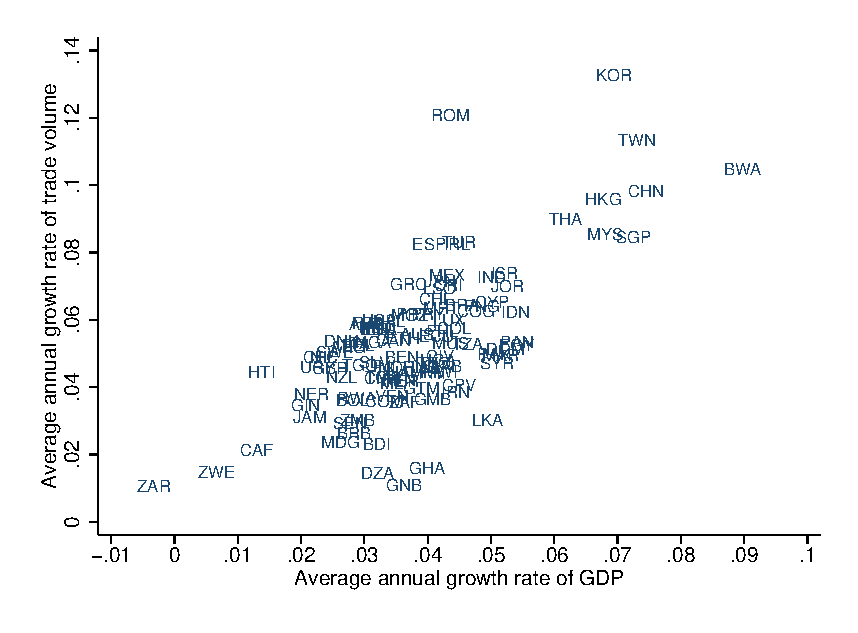
\includegraphics[scale=1.2]{figure_1_5.eps}
\end{center}
}



\end{document}